% Created 2020-02-26 Wed 23:29
% Intended LaTeX compiler: pdflatex
\documentclass[a4paper, 11pt]{extarticle}
             \usepackage[utf8]{inputenc}
\usepackage[left=2cm, right=2cm, bottom=2.5cm, top=2.5cm]{geometry}
% Paquetes de matemáticas
\usepackage{amsmath, amsfonts, amssymb, commath}
\usepackage{tikz}
\usepackage{tikz-cd}
\newcommand{\tikzcircle}[2][red,fill=red]{\tikz[baseline=-0.5ex]\draw[#1,radius=#2] (0,0) circle ;}%
% Ajustes de idioma, gráficos, etc
\usepackage{adjustbox}
\usepackage{float}
\usepackage{hyperref}
\usepackage{graphicx}
\usepackage{gensymb}
\usepackage[spanish, english]{babel}
\usepackage{tikz}
\usepackage{multicol}
\usepackage{listings}
\usepackage{enumitem}
\setlist{nolistsep}
\usepackage{booktabs}
\usepackage{xcolor}
\usepackage{wrapfig}
%Fuentes.
% Alegreya tiene este toque antiguo con serifa, y la tipografía de las ecuaciones es también interesante.
% Gillius no tiene serifa, y también es equilibrada.
\usepackage[T1]{fontenc}
%\usepackage[default]{gillius}
\usepackage{newpxtext, newpxmath}
% Paquete para añadir Creative Commons al final del documento
\usepackage[
type={CC},
modifier={by-nc-nd},
version={3.0},
]{doclicense}
% Propiedades de párrafo
\setlength{\parindent}{0em}
\setlength{\parskip}{1.1em}
\renewcommand{\baselinestretch}{1.05}
\setlength\itemsep{0em}
% Definición de comandos. Muchos de ellos han surgido para Geometría, aunque se
% irá actualizando la lista. POSIBLEMENTE LO INTRODUZCA COMO COMANDOS DE ORG
\newcommand{\m}{\text{medio}}
\newcommand{\iso}{\text{Isom}}
% Para incluir mathcal en las ecuaciones. El /mathcal para Alegreya es el viejo
% y floritural estilo que odio.
\usepackage{calrsfs}
\DeclareMathAlphabet{\pazocal}{OMS}{zplm}{m}{n}
% Definición de colores agradables a la vista
\definecolor{azul}{HTML}{107896}
\definecolor{naranja}{HTML}{C2571A}
\definecolor{rojo}{HTML}{9A2617}
\definecolor{amarillo}{HTML}{BCA136}
\definecolor{verde}{HTML}{829356}
\definecolor{gris}{HTML}{909090}
\definecolor{rosa}{HTML}{F9A7B0}
\definecolor{amarillochillon}{HTML}{FBB117}
% Definición de comandos para teoremas, etc. El comando también incluye
% como argumento un texto, del estilo Teorema 3.5
\newcommand{\axioma}[1]{\textcolor{naranja}{\textbf{Axioma #1}}}
\newcommand{\tma}[1]{\textcolor{rojo}{\textbf{Teorema #1}}}
\newcommand{\propo}[1]{\textcolor{rojo}{\textbf{Proposición #1}}}
\newcommand{\defi}[1]{\textcolor{azul}{\textbf{Definición #1}}}
\newcommand{\obs}[1]{\textcolor{verde}{\textbf{Observación #1}}}
\newcommand{\ejem}[1]{\textcolor{verde}{\textbf{Ejemplo #1}}}
\newcommand{\ej}[1]{\textcolor{amarillo}{\textbf{Ejercicio #1}}}
\newcommand{\lema}[1]{\textcolor{rosa}{\textbf{Lema #1}}}
\newcommand{\cor}[1]{\textcolor{rosa}{\textbf{Corolario #1}}}
% La demostración es igual pero va con una letra más pequeña y en gris.
\newcommand{\dem}[1]{\textcolor{gris}{\small{Demostración. #1}}}
% Esto pone un triangulito de peligro para cuando algo es importante.
\newcommand{\importante}{\tikzcircle[amarillo, fill=amarillo]{4pt}\,}
% Para usar columnas emplea este trozo de código
% \begin{multicols*}{2}
% [\section{Axiomas para la geometría euclidiana plana}]
% 	\axioma{P1} Si tenemos el conjunto $\P$, denominado \textbf{plano}, y la aplicación $d:\P \times \P \rightarrow \R$ llamada \textbf{distancia}, entonces$(\P, d)$ es un espacio métrico.

\defi{2.2} Una \textbf{recta} $r \subset \P$ satisface
\begin{itemizex}
	\item $r$ contiene al menos dos puntos.
	\item Para toda terna de puntos $A, B, C$, están alineados si están en $r$.
\end{itemizex}

\axioma{P2} $\P$ contiene al menos tres puntos no alineados; y por dos puntos distintos, $A$ y $B$ de $\P$ pasa una recta, $r_{AB}$.

\defi{2.6} / \tma{2.7} Dos rectas se cortan si sólo tienen un punto en común, y si no tienen ningún punto en común, entonces se denominan \textbf{paralelas}, y se denota por $a \parallel b$. Dos rectas, o se cortan o son paralelas.

\importante\axioma{P3} Para toda recta $r \subset \P$ existe una biyección $\gamma: r \rightarrow \R$ tal que $|\gamma(X) - \gamma(Y)| = |x - y| = d(X, Y) \;\; \forall \;\; X,Y \in r$ 

\obs{2.8} Si $A, B \in r$ son distintos, entonces existe un punto $M\in r: d(A,M) = d(M,B)$ que denotamos por $\m[A,B]$ y se llama \textbf{punto medio}. Asimismo sólo existe un punto $B \in r$ tal que $B = \m[A, M]$.

\obs{2.9} Si $r$ es una recta y $P \in r$, entonces $r$ se puede dividir en dos \textbf{semirrectas}, que son los conjuntos $\{X \in r \; | \; \gamma(X) > \gamma(P)\}$ y $\{X \in r \; | \; \gamma(X) < \gamma(P)\}$.

\axioma{P4} Para toda recta $r \subset \P$ hay dos subconjuntos $H^1$ y $H^2$, denominados \textbf{semiplanos} de $r$, que verifican:
\begin{itemizex}
	\item $H^1 \cup H^2 = \P-r$
	\item Si $X,Y \in H^i$ entonces $[X,Y] \subset H^i$
	\item Si $X \in H^1$ y $Y \in H^2$ entonces $[X,Y] \cap r \neq \emptyset$.
\end{itemizex}

\defi{2.15} Sean $P, Q, R$ no alineados, entonces el triángulo $\triangle\{P,Q,R\}$, o $\triangle PQR$ está formado por los segmentos $[P,Q]$, $[Q,R]$, $[P,R]$, llamados lados, y los vértices $P,Q, R$.

\tma{2.16 [Axioma de Pasch]a} Dado un triángulo $\triangle PQR$ y una recta $r$; si $r$ corta a $[P,Q]$, entonces o corta a $[P,R]$ o a $[Q, R]$.

\defi{2.17 = 1.5} Una \textbf{isometría} en $\P$ es una biyección $g: \P \rightarrow \P$ que cumple que $d(g(X), g(Y)) = d(X,Y) \;\;\forall\;\; X,Y \in \P$.

\tma{2.18} Si $A,B \in \P$ y $g \in \iso(\P)$ entonces $g([A,B]) = [g(A), g(B)]$ y $g(r_{AB}) = r_{g(A)g(B)}$ 

\axioma{P5} Si $A_1, A_2 \in \P$ y $B_1, B_2 \in \P$ son dos pares de puntos que cumplen $d(A_1,A_2) = d(B_1,B_2)$ entonces existe $g \in \iso(\P)$ tal que $g(A_i) = B_i$. Se dice que esos pares de puntos son \textbf{congruentes}.

\axioma{P6} Para toda recta $r$ existe una isometría $\sigma$ llamada \textbf{reflexión} tal que  
\begin{itemizex}
	\item $\sigma(X) = X\iff X \in r$
	\item $\sigma \circ \sigma = \text{Id}$
\end{itemizex}


\defi{2.23} / \tma{2.25} / \cor{2.30} Una recta $l$ es \textbf{ortogonal} a $r$ si para todo $S \in l$ y para todo par de puntos $A, B$ que cumple que $M = \m[A,B]$, de modo que $l \cap r = M$, entonces se da que $d(A,S) = d(S,B)$. Se denota $l \perp_M r$. En estas condiciones, $l = \{X \in \P \; | \; d(S,A) = d(S,B)\}$, se denomina \textbf{mediatriz} de $[A,B]$. 

\begin{figure}[H]
	\centering
	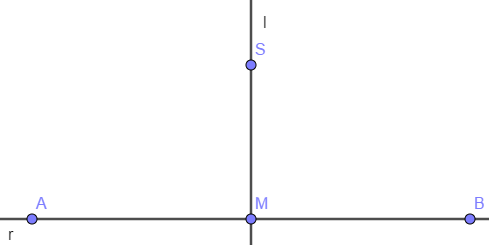
\includegraphics[width=7cm]{figuras/2-23.png}
	\vspace{-1em}
\end{figure}

\lema{2.21} Si $\sigma_r$ entonces, para todo $X$, $\m[X, \sigma_r(X)] \in r$.

\obs{2.24} Si $l \perp r$ y $g \in \iso(\P)$ entonces $g(l) \perp g(r)$.

\importante\tma{2.26} Si $l, r \subset \P$ cortan en $M$ y $\sigma_l, \sigma_r$ son dos reflexiones de $l$ y $r$, entonces se cumple que $l \perp_M r \iff r \perp_M l \iff \sigma_r(l) = l \iff \sigma_l(r) = r$.

\importante\tma{2.27 / 2.29} Para toda recta $r$ y todo punto $S \in \P - r$, existe una recta $l$ ortogonal a $r$, que pasa por $S$. Si $r$ es una recta, y $M \in r$, entonces existe $l$ tal que $l \perp_M r$.

\axioma{P7} Para toda recta $r$ y todo punto $P$ existe sólo una recta \textbf{paralela} a $r$ que pase por $P$.

\tma{2.31 / 2.33} Si $a \perp l$ y $b \perp l$ entonces $a \parallel b$. Sean $a \parallel b$. Entonces, para todo $A \in a$, la única recta $l \perp_A a$ también es ortogonal a $b$.

\tma{2.32} Las rectas parallelas forman una relación de equivalencia.
\begin{itemizex}
	\item Reflexividad: $a\parallel a$
	\item Simetría: $a \parallel b \rightarrow b \parallel a$
	\item Transitividad  $a \parallel b $ y  $b \parallel c \rightarrow a \parallel c$
\end{itemizex}

\ej{2.6} Sean $A,B \in r$, $A \neq B$. Para todo $t$, existe un único $P_t\in r$ que cumple $d(P_t,A) = \abs{t}$ y $d(P_t, B) = \abs{t-d(A,B)}$. En definitiva, la posición de $P_t$ está sólamente determinada por las distancias $d(A, P_t)$ y $d(P_t, B)$.
	 
	 
	 
	 
	 
	 
	 \end{multicols*}\pagebreak
% multicols* obliga a terminar una columna antes de empezar la siguiente.
\DeclareMathAlphabet{\pazocal}{OMS}{zplm}{m}{n}
\let\mathcal\pazocal
\usepackage{fancyhdr}
\pagestyle{fancy}
\lhead{Alex Martínez Ascensión}
\chead{}
\rhead{\today}
\date{}
\title{\Huge\vspace{-1em}Variable compleja}
\hypersetup{
 pdfauthor={},
 pdftitle={\Huge\vspace{-1em}Variable compleja},
 pdfkeywords={},
 pdfsubject={},
 pdfcreator={Emacs 26.2 (Org mode 9.2.5)}, 
 pdflang={English}}
\begin{document}

\maketitle
\vspace{-8em}

\section*{Los números complejos}
\label{sec:org0d97ac7}
\begin{multicols}{2}

\defi{1.1} Un número complejo es una expresión \(a + bi\) donde 
\(a,b \in \mathbb{R}\) y \(i\) es la unidad imaginaria, fruto de resolver la
ecuación \(x^2 + 1 = 0\) en \(\mathbb{R}\). Así, definimos \(i = \sqrt{-1}\). Si \(z \in \mathbb{C} = a + bi\), \(a = \text{Re }z\) y \(b = \text{Im
}z\) son la parte \textbf{real} e \textbf{imaginaria} de \(z\).

\defi{1.2} La \textbf{suma} y \textbf{multiplicación} están definidas en los complejos así:
\[ \left(x_{1}+y_{1} i\right)+\left(x_{2}+y_{2}
i\right)=\left(x_{1}+x_{2}\right)+\left(y_{1}+y_{2}\right) i \]
$$
\left(x_{1}+y_{1} i\right)\left(x_{2}+y_{2} i\right)=\left(x_{1} x_{2}-y_{1} y_{2}\right)+\left(x_{1} y_{2}+x_{2} y_{1}\right) i
$$
Y con estas operaciones \((\mathbb{C}, +, \cdot)\) es un cuerpo, con \(0_{\mathbb{C}} = 0 + 0i\) y \(1_\mathbb{C} = 1 + 0i\).

\defi{1.3} Dado un complejo \(z = x + yi\), llamamos \textbf{conjugado} de \(z\), \(\oveline{z}\) a \(x - yi\).

\propo{1.3.1} Se verifica que \(\overline{z_{1}+z_{2}}=\overline{z_{1}}+\overline{z_{2}}\) 
y \(\overline{z_{1} z_{2}}=\overline{z_{1}} \cdot \overline{z_{2}}\).

\defi{1.4.1} Se denomina \textbf{módulo} de un complejo \(z = x + yi\), \(|z|\) a \(\sqrt{x^2 + y^2}\). Se cumple que \(|z| = \sqrt{z\overline{z}}\). 
El módulo cumple que (1) \(|z| \ge 0\), (2) \(|z| = 0 \iff z = 0\),
(3) \(|z_1z_2| = |z_1||z_2|\) y (4) \(|z_1 + z_2| \le |z_1| + |z_2|\)

\dem{ (4) \( 
\left|z_{1}+z_{2}\right|^{2}=\left(z_{1}+z_{2}\right)(\overline{z_{1}+z_{2}})=\left(z_{1}+z_{2}\right
)(\overline{z_{1}}+\overline{z_{2}}) 
=z_{1} \overline{z_{1}}+z_{1} \overline{z_{2}}+z_{2} \overline{z_{1}}+z_{2} \overline{z_{2}} 
=z_{1} \overline{z_{1}}+z_{1} \overline{z_{2}}+\overline{z_{1} \overline{z_{2}}}+z_{2} \overline{z_{2}} 
=\left|z_{1}\right|^{2}+\left|z_{2}\right|^{2}+2 \operatorname{Re}\left(z_{1} \overline{z_{2}}\right) 
 \leq\left|z_{1}\right|^{2}+\left|z_{2}\right|^{2}+2\left|z_{1}\right|\left|z_{2}\right| 
=\left(\left|z_{1}\right|+\left|z_{2}\right|\right)^{2}
 \)  }

\defi{1.5} Dado un \(z = a + bi\), aplicando \(u = p + iq = z/|z|\),
entonces \(|u| = 1 = p^2 + q^2\). El ángulo tal que \(p = \cos \alpha, q =
\sin \alpha\) se denomina \textbf{argumento}, \(\arg z\).  Así, \(z\) puede representarse como \(z
= |z|(\cos  \alpha  + i \sin \alpha )\). Esta forma es la \textbf{forma polar}, y
también se representa como \(z = |z|e^{i\alpha}\).x 

El argumento cumple que (1) \(\arg \overline{z} = - \arg z\) y (2) \(\arg
z_1z_2 = \arg z_1 + \arg z_2\).

\defi{1.7 / 1.8} El espacio topológico \((\mathbb{C}, \delta_E)\) con distancia
euclídea no es compacto. Sin embargo, si tomamos \(\hat{\mathbb{C}} =
\mathbb{C} \cup \{ \infty \}\) entonces sí es compacto, y lo denominamos \textbf{plano
complejo ampliado}. La \textbf{esfera de Riemann}, \(\mathbb{S}\), es la representación del conjunto \(\hat{\mathbb{C}}\) en \(\mathbb{R}^3_{(\xi, \eta, \zeta)}\) en una esfera con
centro \((0, 0, 1/2)\) con ecuación \(\xi^{2}+\eta^{2}+\zeta^{2}-\zeta=0\).
\begin{figure}[H]
\centering
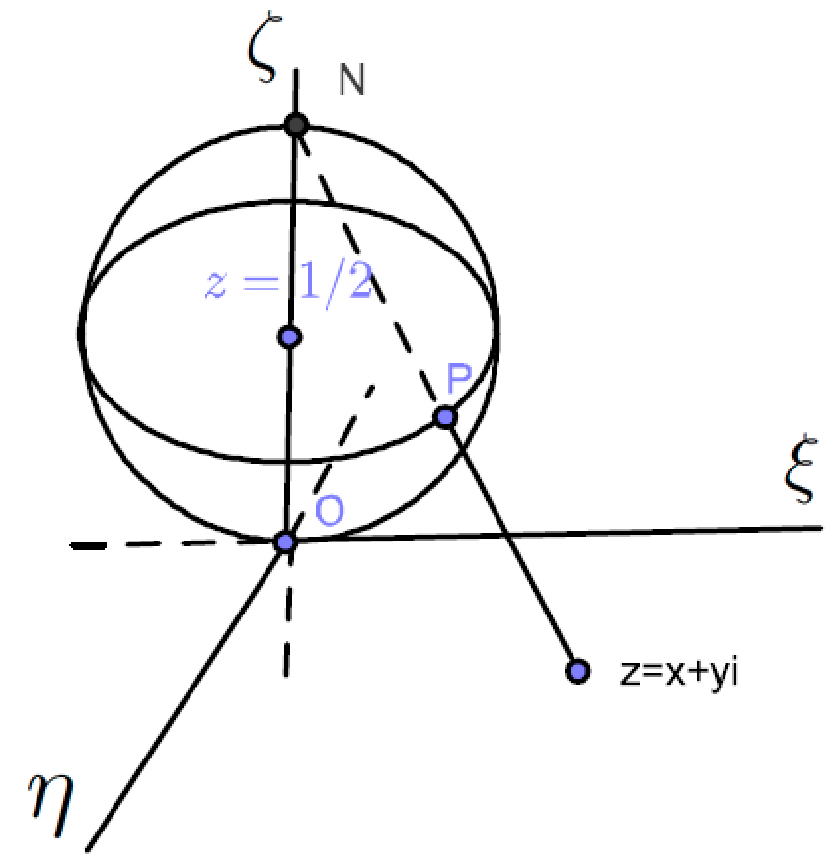
\includegraphics[width=5cm]{imagenes/esfera.png}
\end{figure}
La relación entre la esfera y el plano es 
\[ \xi=\frac{x}{1+x^{2}+y^{2}}, \eta=\frac{y}{1+x^{2}+y^{2}}, \zeta=\frac{x^{2}+y^{2}}{1+x^{2}+y^{2}} \]
La \textbf{distancia cordal} entre dos puntos \(z_1,z_2\) es la distancia euclídea 
entre los puntos \(P_1,P_2\) de la esfera de la esfera de Riemman.

\(\delta(z_1,z_2) =
 \sqrt{\left(\xi_{1}-\xi_{2}\right)^{2}+\left(\eta_{1}-\eta_{2}\right)^{2}+\left(\zeta_{1}-\zeta_{2}\right)^{2}}
 = \frac{\sqrt{\left(x_{1}-x_{2}\right)^{2}+\left(y_{1}-y_{2}\right)^{2}}}{
\sqrt{\left(1+x_{1}^{2}+y_{1}^{2}\right)\left(1+x_{2}^{2}+y_{2}^{2}\right)}}\)

Para un punto en el infinito, la distancia es \(\delta(z, \infty)=\frac{1}{\sqrt{1+x^{2}+y^{2}}}\)

\end{multicols}
\pagebreak




\section*{Funciones complejas}
\label{sec:org6e3dcf2}
\begin{multicols}{2}
\defi{2.0} Una función puede ser de tipo \(f: \mathbb{R} \rightarrow
\mathbb{C}\) (f. compleja de var. real) o 
\(f: \mathbb{C} \rightarrow  \mathbb{C}\) (f. compleja de var. compleja).

\defi{2.1.1} \(f = f(z)\) es \textbf{continua} en \(z_0 \in \mathbb{C}\) si para todo \(\epsilon > 0\) existe \(\delta > 0\) tal que si \(|z - z_0| < \delta\)
entonces \(|f(z) - f(z_0)| < \epsilon\). \(f\) es \textbf{uniformemente continua} en
\(B \subset \mathbb{C}\) si
dado \(\epsilon > 0\) existe \(\delta > 0\) tal que para todo \(z_0 \in B\) y para todo \(z\) tal que \(|z-z_0| < \delta\) entonces \(|f(z) -
f(z_0)| < \epsilon\).  Si \(f\) es uniformemente continua es continua, pero
no siempre a la inversa.

\tma{2.1.1} Si \(f_1(z), f_2(z)\) están definidas en \(A \subset \mathbb{C}\), \(A\) abierto, y son continuas en \(z_0 \in A\), f\textsubscript{1} + f\textsubscript{2} y f\textsubscript{1}/f\textsubscript{2} son
continuas en \(z_0\). Así, los polinomios complejos son continuos.

\defi{2.1.2} Una función \(f(z)\) en \(A \subset \mathb{S}\) es continua en
\(z_0\) si para todo \(\epsilon > 0\)
 existe \(\eta > 0\) tal que para todo \(z \in A\) donde \(\delta(z, z_0) <
\eta\) entonces \(\delta(f(z_0), f(z)) < \epsilon\).

\defi{2.2.1, 2.2.2} Una función \(f(z)\) es \textbf{derivable} en \(z_0\) si existe el
límite \(\lim_{z \to z_0} \frac{f(z) - f(z_0)}{z-z_0}\) y es finito.
Si \(z_0 = \infty\), consideramos \(g(z) = f(1/z)\) y \(f\) es derivable
en \(\infty\) si \(g\) es derivable en \(z=0\).
Una función \(f:A\sub \mathbb{C} \rightarrow  \mathbb{C}\) derivable en todo
\(A\) se llama función \textbf{holomorfa} o \textbf{analítica.}

\propo{2.3.2} Si \(f\) es derivable en un punto, también es continua en ese
punto.

\propo{2.3.4 (Regla de la cadena)} Sean \(g:A \rightarrow  \mathbb{C}\) y \(f: B \rightarrow \mathbb{C}\) tal que \(g(A) \subset B\). Si \(g\) es
derivable en \(z_0\) y \(f\) es derivable en \(g(z_0)\) entonces \(f
\circ g'(z_0) = f'(g(z_0))g'(z_0)\).


\end{multicols}
\pagebreak
\end{document}